\documentclass[12pt]{beamer}

\usepackage[utf8]{inputenc}
\usepackage[T1]{fontenc}
\usepackage[ngerman]{babel}
\usepackage{amsmath}
\usepackage{amssymb}
\usepackage{csquotes}
\usepackage{hyperref}
\usepackage{algorithm}
\usepackage{algpseudocode}
\usepackage{graphicx}
\usepackage{wrapfig}
\usepackage{tikz}
\usepackage{circuitikz}
\usepackage{tikz-timing}
\usepackage{bytefield}
\usepackage{pgf-umlcd}
\usepackage[backend=biber, style=ieee, citestyle=ieee]{biblatex}
\usepackage{rotating}
\usepackage{colortbl}

\usetikzlibrary{positioning,trees}

\usetikztiminglibrary{advnodes,either,beamer,overlays}


\usetheme{Madrid}
\usecolortheme{whale}

\newcounter{listnum}

\title{Mikrocontroller Touchscreen GUI}
\author{Neo Hornberger, Tim Ludwig}
\date{21.01.2022}

\bibliography{../Bibliography.bib}

\begin{document}
	\maketitle
	
	\section{Touchscreen Hardware}
	\frame{\tableofcontents[currentsection]}
	
	\begin{frame}{Resistive Touchscreens}
		\begin{columns}
			\begin{column}{0.4\textwidth}
				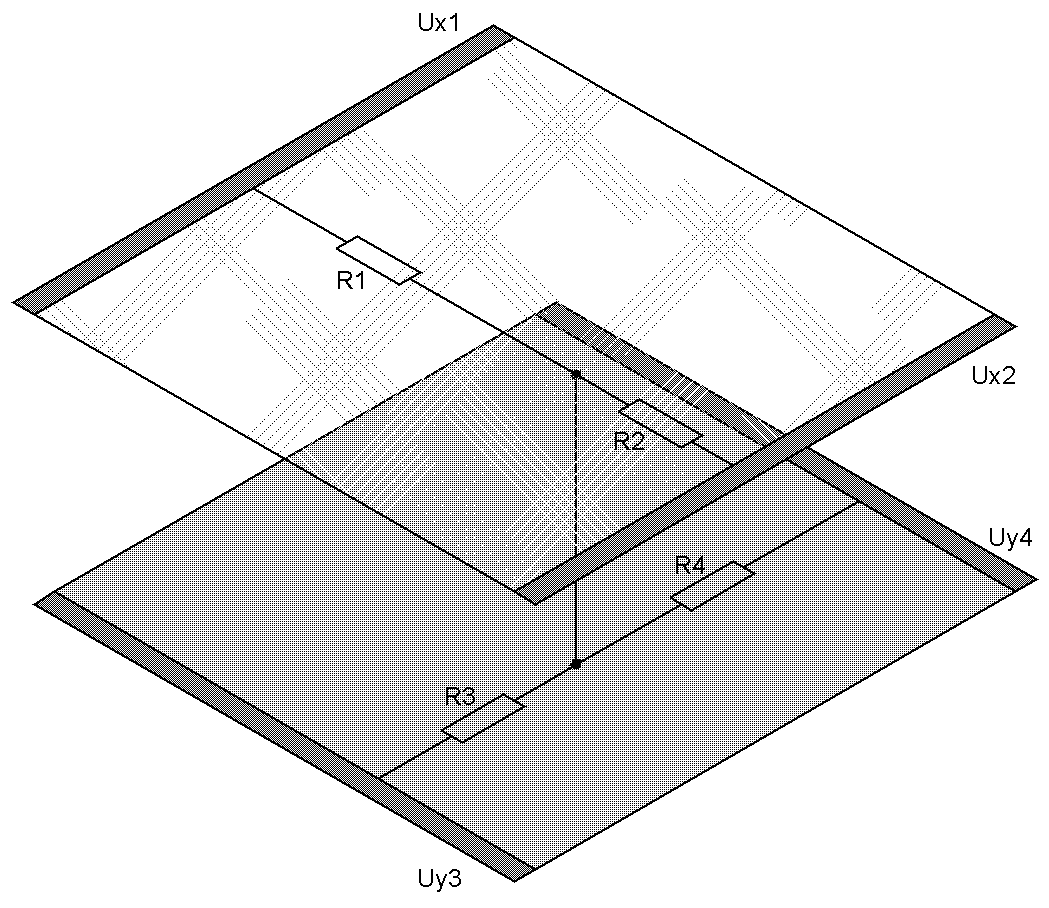
\includegraphics[width=\textwidth]{../Images/ResistiveTouchScreen.png}
			\end{column}
			\begin{column}{0.6\textwidth}
				Funktionsweise: 
				\begin{itemize}
					\item<1-> Kontakt zweier Schichten durch Deformierung
					\item<2-> Anlegen einer Spannung über eine Schicht
					\item<3-> Messen des Potentials an den Enden der anderen Schicht
					\item<4-> Wdh. mit vertauschten Rollen
				\end{itemize}
				
				Häufige Nutzung:
				\begin{itemize}
					\item Kiosksysteme
					\item Industrie
					\item \dots
				\end{itemize}
			\end{column}
		\end{columns}
	\end{frame}

	\begin{frame}{kapazitive Touchscreens}
		Arten von kapazitiven Touchscreens:
		\begin{itemize}
			\item Oberflächen-kapazitiv
			\item Projiziert-kapazitiv
		\end{itemize}
		\medskip
		Häufige Nutzung:
		\begin{itemize}
			\item Smartphones
			\item Tablets
			\item \dots
		\end{itemize}
	\end{frame}

	\begin{frame}{Oberflächen-kapazitive Touchscreens}
		\begin{columns}
			\begin{column}{0.4\textwidth}
				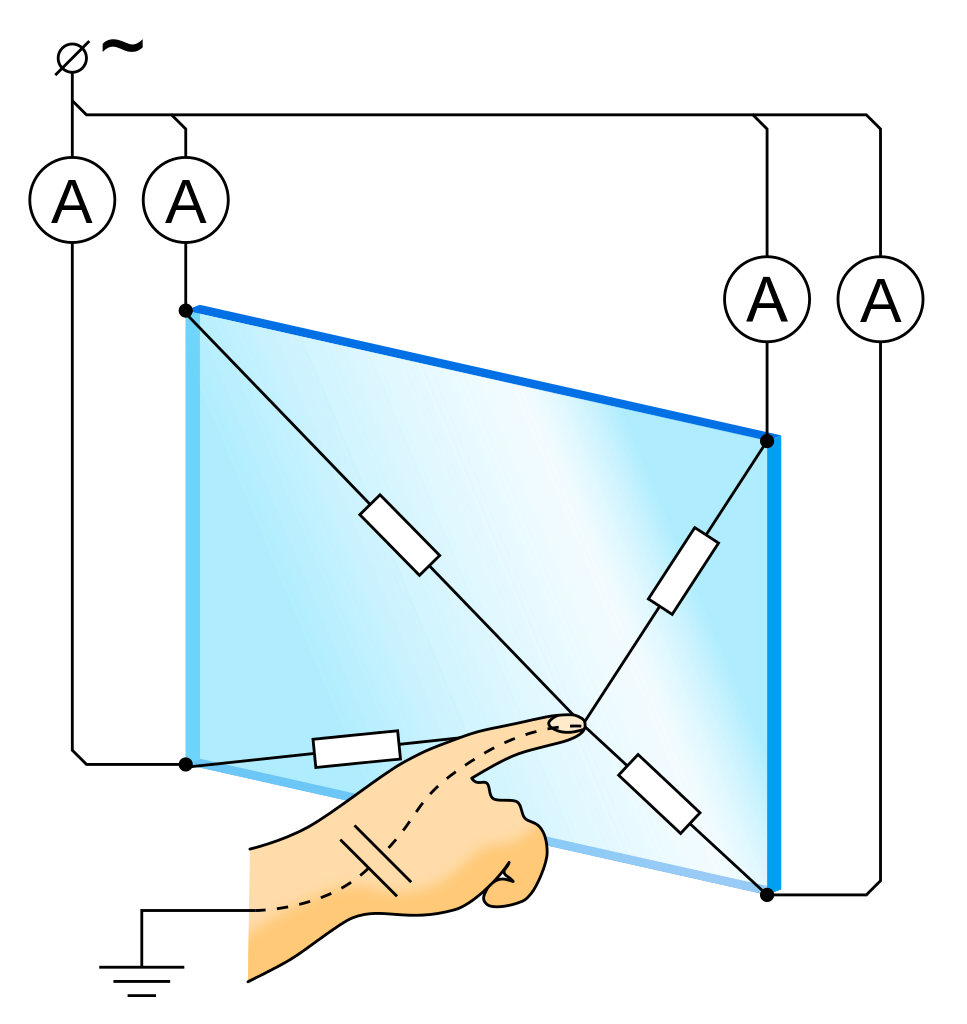
\includegraphics[width=\textwidth]{../Images/SurfaceCapacitiveTouchScreen.png}
				
			\end{column}
			\begin{column}{0.6\textwidth}
				Funktionsweise:
				\begin{itemize}
					\item<1-> Wechselspannung an den Ecken anlegen
					\item<2-> bei Berührung wird eine Kapazität auf- und entladen
					\item<3-> den Strom durch die Ecken messen
				\end{itemize}
			\end{column}
		\end{columns}
	\end{frame}
	
	\begin{frame}{Projiziert-kapazitive Touchscreens}
		\begin{columns}
			\begin{column}{0.4\textwidth}
				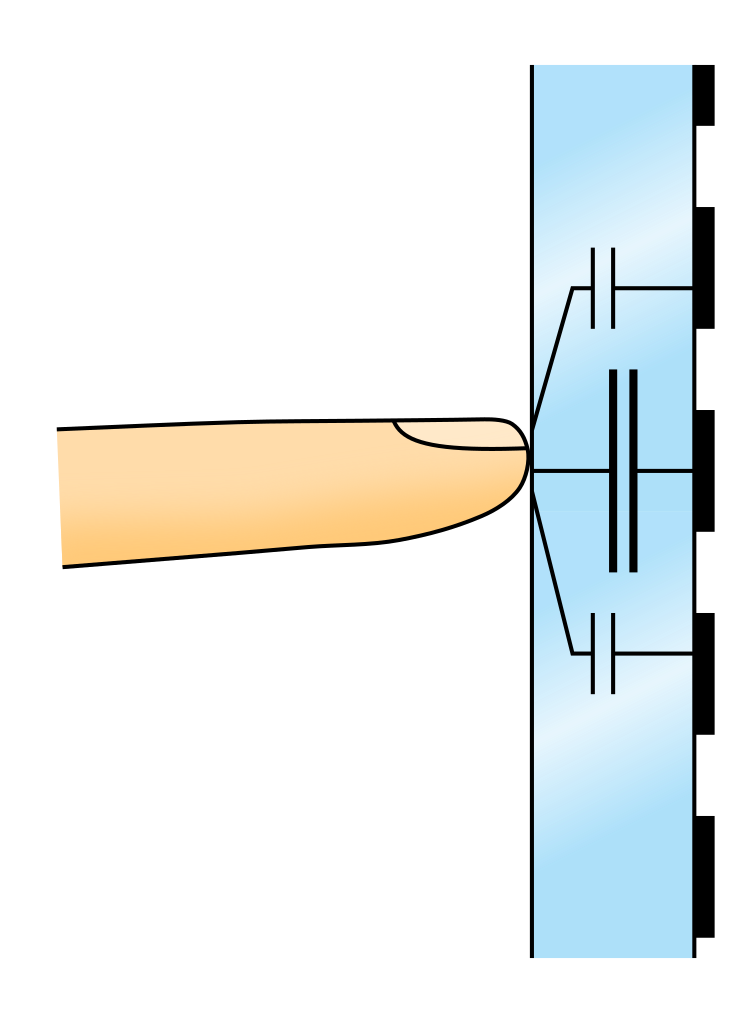
\includegraphics[width=\textwidth]{../Images/ProjectedCapacitiveTouchScreen.png}
			\end{column}
			\begin{column}{0.6\textwidth}
				Funktionsweise:
				\begin{itemize}
					\item<1-> zwei Ebenen Gitter aus Leitern
					\item<2-> Anlegen einer Wechselspannung an eine Ebene
					\item<3-> Messen des durch die Leiter der anderen Ebene fließenden Stroms
				\end{itemize}
			\end{column}
		\end{columns}
	\end{frame}
	
	\begin{frame}{Kapazitiv vs. Resistiv}
		\begin{tabular}{| >{\columncolor{structure.fg!80}\color{white}} l | p{4.5cm} | p{4.5cm} |}
			\hline
			\rowcolor{structure.fg!80} & \color{white}Vorteile & \color{white}Nachteile\\\hline
			kapazitiv & \normalcolor
				\begin{itemize}
					\item geringer Verschleiß
					\item Multitouch
				\end{itemize} &
				\begin{itemize}
					\item leitendes Material (Finger, spez. Stifte, \dots) notwendig
					\item Kalibration
				\end{itemize}\\\hline
			resistiv &
				\begin{itemize}
					\item ohne leitendes Material bedienbar
					\item unempfindlich gegenüber Staub, Wasser, \dots
				\end{itemize} &
				\begin{itemize}
					\item erhöhter Verschleiß
					\item unerwünschtes Auslösen
				\end{itemize}\\\hline
		\end{tabular}
	\end{frame}

	\section{I²C}
	\frame{\tableofcontents[currentsection]}
	
	\begin{frame}{Der I²C-Bus}
		\begin{itemize}
			\item Bussystem bestehend aus zwei Leitungen (\texttt{SDA}, \texttt{SCL})
			\item Aufteilung der Daten in Bytes (8-Bit-Wörter)
			\item Versenden der Bytes in MSB-Bitreihenfolge
			\item Komponenten besitzen eine 7-Bit Adresse
			\item Controller/Target-Prinzip
			\item nach jedem gesendeten Byte bestätigt der Empfänger dies
		\end{itemize}
	\end{frame}
	
	\begin{frame}{Kommunikationsstart}
		\begin{columns}
			\begin{column}{0.45\textwidth}
				\texttt{Controller}:
				\begin{enumerate}
					\item Startanweisung (\texttt{START})
					\item 7-Bit Adresse
					\item R/$\overline{\mbox{W}}$-Bit
					
					\setcounter{listnum}{\value{enumi}}
				\end{enumerate}
				\texttt{Target}:
				\begin{enumerate}
					\setcounter{enumi}{\value{listnum}}
					
					\item Bestätigung (\texttt{ACK})
				\end{enumerate}
			\end{column}
			\begin{column}{0.5\textwidth}
				\begin{figure}
	\begin{tikztimingtable}
		% width=11.375
		%
		SDA & H L E 6{D{}} E L .375H ; [dotted] h \\
		SCL & 1.5H .875C {c N(c1) c} {c N(c2) c} {c N(c3) c} {c N(c4) c} {c N(c5) c} {c N(c6) c} {c N(c7) c} {c N(c8) c} {c N(c9) c} ; [dotted] l \\
		%
		\begin{extracode}[every node/.style={font=\tiny}]
			\foreach \i in {1,...,9}
				\node[left=-.345em of c\i.mid](\i){\i};
		\end{extracode}
	\end{tikztimingtable}
\end{figure}

			\end{column}
		\end{columns}
	\end{frame}

	\begin{frame}{Übertragung von Daten}
		\begin{columns}
			\begin{column}{0.45\textwidth}
				Sender:
				\begin{enumerate}
					\item 8-Bit Wort
					
					\setcounter{listnum}{\value{enumi}}
				\end{enumerate}
				
				Empfänger:
				\begin{enumerate}
					\setcounter{enumi}{\value{listnum}}
					
					\item Bestätigung (\texttt{ACK})
				\end{enumerate}
				
				\vspace{5ex}
				Wdh. bis alle Bytes versendet sind.
			\end{column}
			\begin{column}{0.5\textwidth}
				\begin{tikztimingtable}
	% width=9.625
	%
	SDA & ; [dotted] h ; .25H E 6{D{}} E N(ackL) L N(ackR) .375H ; [dotted] h \\
	SCL & ; [dotted] l ; .625L {c N(c1) c} {c N(c2) c} {c N(c3) c} {c N(c4) c} {c N(c5) c} {c N(c6) c} {c N(c7) c} {c N(c8) c} {c N(c9) c} ; [dotted] l \\
	%
	\begin{extracode}[every node/.style={font=\tiny}]
		\foreach \i in {1,...,9}
			\node[left=-.345em of c\i.mid] (\i) {\i};
		
		\begin{pgfonlayer}{background}
			\draw[draw=gray,dashed] ([shift={(-.075,-2.5)}] ackL.LOW) rectangle ([shift={(.125,.5)}] ackR.high);
			\node[color=gray,below left=.5ex and .25em of c9.low,anchor=north] {\texttt{ACK}};
		\end{pgfonlayer}
	\end{extracode}
\end{tikztimingtable}

			\end{column}
		\end{columns}
	\end{frame}

	\begin{frame}{Kommunikationsende}
		\begin{columns}
			\begin{column}{0.55\textwidth}
				\texttt{Controller}:
				\begin{enumerate}[a]
					\item Stopanweisung (\texttt{STOP})
					\item erneute Startanweisung (\texttt{repeated START})
				\end{enumerate}
			\end{column}
			\begin{column}{0.4\textwidth}
				\begin{figure}
	\begin{tikztimingtable}
		% width=2
		%
		SDA & ; [dotted] .25E .75L ; L H \\
		SCL & ; [dotted] .75E .25C ; 2H \\
	\end{tikztimingtable}
\end{figure}

				\begin{figure}
	\begin{tikztimingtable}
		SDA & ; [dotted] .5H ; .75H L \\
		SCL & ; [dotted] .5L ; .25L 1.5H \\
	\end{tikztimingtable}
\end{figure}

			\end{column}
		\end{columns}
	\end{frame}
	
	\section{Software}
	\frame{\tableofcontents[currentsection]}
	
	\begin{frame}{Planung \& Entwurfsziele}
		Implementation typischer Touchscreen GUI Komponenten in C++.
		
		\begin{itemize}
			\item Radio Button
			\item Toggle Switch
			\item Slider
			\item Button
			\item Check Box
		\end{itemize}
		\pause
		\bigskip
		\begin{itemize}
			\item leicht benutzbar $\Rightarrow$ orientiert an typischen Design Guidelines \cite{material-components} \pause
			\item leicht programmierbar $\Rightarrow$ viel Abstraktion, wenig Boilerplate \pause
			\item möglichst Ressourcen schonend $\Rightarrow$ Abfragen und zeichnen auf einer \emph{need-to-know} Basis
		\end{itemize}
	\end{frame}

	\begin{frame}{Komponenten}
		\centering\begin{tikzpicture}[sibling distance=7em,
	every node/.style = {shape=rectangle, rounded corners,
		draw, align=center}]
	\node {TouchScreen}
		child { node {RootContainer}
			child { node {Switch}}
			child { node {Switch}}
			child { node {Container}
				child { node {RadioButton}}
				child { node {RadioButton}}
				child { node {RadioButton}}
			}
			child { node {Slider}}
		};
\end{tikzpicture}
	\end{frame}

	\begin{frame}{Das Event System}
		\begin{columns}
			\begin{column}{0.6\textwidth}
				\begin{tikzpicture}[y=-1cm]
	\node[draw](root){RootContainer};
	\node[draw=gray,color=gray,below right=1em of root,anchor=north west](slider){Slider};
	\node[draw=gray,color=gray,below right=1em of slider,anchor=north west](listener1){Listener 1};
	\node[draw,below left=6ex and 0em of slider,anchor=north west](switch){Switch};
	\node[draw,below right=1em of switch,anchor=north west](listener2){Listener 2};
	\node[draw,below left=1ex and 0em of listener2,anchor=north west](listener3){Listener 3};
	
	
	\draw[-latex,color=gray] (root.south) |- (slider);
	\draw[-latex,color=gray] (slider.south) |- (listener1);
	\draw[-latex] (root.south) |- (switch);
	\draw[-latex] (switch.south) |- (listener2);
	\draw[-latex] (switch.south) |- (listener3);
\end{tikzpicture}
			\end{column}
			\begin{column}{0.4\textwidth}
				\pause
				Berührung außerhalb der \emph{Bounding-Box} von \texttt{Slider}.
			\end{column}
		\end{columns}
		
	\end{frame}

	\section{Quellen}
	\begin{frame}{Quellen}
		\nocite{ts-holzinger}
		\nocite{stm32_refManual}
		\printbibliography
	\end{frame}
\end{document}
